\section{Grundbegriffe}
	\subsection{Einfaches Kommunikationsmodell}
		\begin{center}
			\begin{tikzpicture}[scale=1, transform shape]
\tikzstyle{block} =	[draw, rectangle,
	very thick,
	node distance=3.8cm,
	text width=2cm,
	inner sep = 1ex,
	text centered
	]
\tikzstyle{sum} = [draw, circle,
	very thick,
	node distance = 3.8cm,
	text width=1.1cm, 
	inner sep=1ex, 
	text centered]
\tikzstyle{pfeil} = [draw,
	->, very thick, rounded corners, 
]
    \node [sum]   (source) {Quelle Source};
    \node [block, right of=source]  (sender) {Sender Transmitter};
    \node [block, right of=sender]  (channel) {Kanal Channel}; 
    \node [block, right of=channel] (receiver) {Empfänger Receiver}; 
    \node [sum, right of=receiver]  (sink) {Senke Sink};
    
    \node [block, above=5mm of sender] (noise) {Störung Noise};    
    \draw [pfeil, to path={-| (\tikztotarget)}] 
    	(noise) to (channel);
    	
    \draw [pfeil] (source) -- 
    	node[above=1mm] {Nachricht} 
    	node[below=1mm] {Message}
    	(sender);
    \draw [pfeil] (sender) -- node[above=1mm] {Signal} (channel);
    \draw [pfeil] (channel) -- node[above=1mm] {Signal} (receiver);
    \draw [pfeil] (receiver) -- 
    	node[above=1mm] {Nachricht} 
    	node[below=1mm] {Message}
    	(sink);
\end{tikzpicture}
		\end{center}
\subsection{Signalklassifizierungen}


\renewcommand{\arraystretch}{2}
\begin{tabular}[c]{ | p{9cm} | p{9cm} | }
\hline
	\begin{minipage}[t]{9cm}
		\textbf{Energie} \\
		$ E = W = \lim\limits_{T\rightarrow\infty}\int\limits_{-T/2}^{T/2} |x(t)|^2dt\label{SIG_FORM_01}
		 = \frac{1}{2 \pi} \int\limits_{-\infty}^{\infty} |X(j \omega)|^2 d \omega$ \\
	\end{minipage}
	&
	\begin{minipage}[t]{9cm}
		\textbf{Leistung} \\
		$ P = \lim \limits_{T \to \infty} {\frac{1}{T} \int\limits_{-T/2}^{T/2} {|x(t)|^2 dt}} 
		= \frac{1}{2 \pi} \int\limits_{-\infty}^{\infty} \left( \lim\limits_{T
	\rightarrow \infty} \frac{|X(j \omega)|^2}{T} \right) d \omega	$ \\
	\end{minipage}
	\\
\hline

	\begin{minipage}[t]{9cm}
		\textbf{Energiesignal} - \textit{''Impuls'' bspw. Nachrichtensignal}
		\begin{center}
			$ E < \infty $ \\
			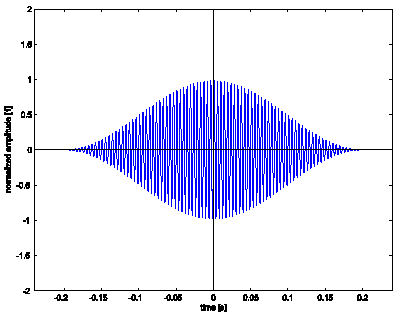
\includegraphics[width=4cm]{bilder/signal_energiesignal.png}
       	\end{center}

	\end{minipage}
	&
	\begin{minipage}[t]{9cm}
		\textbf{Leistungssignal} - \textit{''Dauersignal '' bspw. Trägersignal}
		\begin{center}
			$ E = \infty \text{ und } P < \infty$\\
			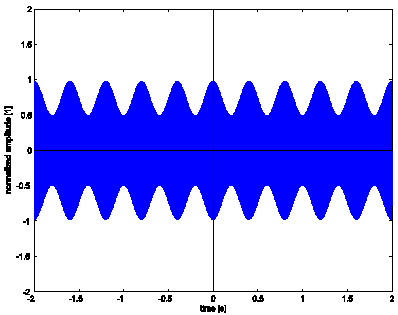
\includegraphics[width=4cm]{bilder/signal_leistungssignal.png}
       	\end{center}

	\end{minipage} \\

\hline

	\begin{minipage}[t]{9cm}
		\textbf{Aperiodisch} \\
		$x(t) \neq x(t + n \cdot T)$
	\end{minipage}
	&
	\begin{minipage}[t]{9cm}
		\textbf{Periodisch} \\
		$x(t) = x(t + n \cdot T) \qquad \text{ mit Periodendauer } T \text { und } n \in \mathbb{Z}$
	\end{minipage}
\\
\hline

	\begin{minipage}[t]{9cm}
		\textbf{Deterministisch} - \textit{mit vorbestimmten Verlauf} \\
		$x(t) = f(t)$
	\end{minipage}
	&
	\begin{minipage}[t]{9cm}
		\textbf{Stochastisch} - \textit{ohne vorbestimmten Verlauf} \\
		$x(t) = ?$
	\end{minipage}
\\
\hline

	\begin{minipage}[t]{9cm}
		\textbf{Zeitkontinuierlich} \\
		$x(t) \text{ ist definiert } \forall t \in \mathbb{R}$
		\begin{center}
			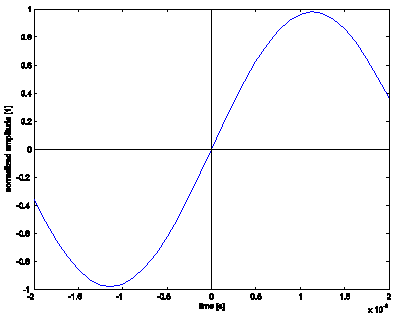
\includegraphics[width=4cm]{bilder/signal_zeitkontinuierlich.png}
       	\end{center}
	\end{minipage}
	&
	\begin{minipage}[t]{9cm}
		\textbf{Zeitdiskret} \\
		$x(t) \text{ nur definiert an Stellen } x(n \cdot T) $ \\
		$  \text{ mit Abtastintervall } T \text { und } n \in \mathbb{Z}$
		\begin{center}
			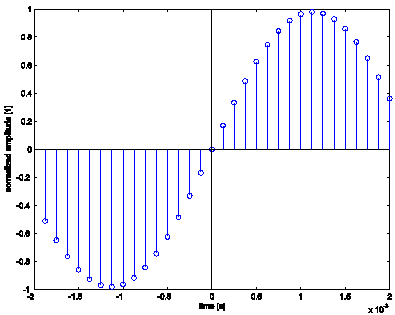
\includegraphics[width=4cm]{bilder/signal_zeitdiskret.png}
       	\end{center}
	\end{minipage}
\\
\hline

	\begin{minipage}[t]{9cm}
		\textbf{Amplitudenkontinuierlich}\\
		$x(t) = y$ mit $y \in \mathbb{R}$
		\begin{center}
			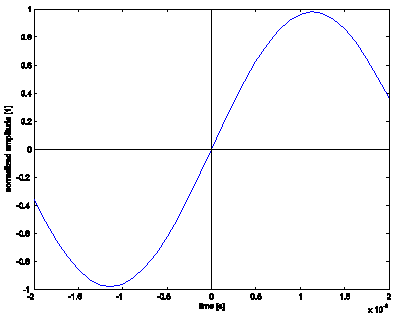
\includegraphics[width=4cm]{bilder/signal_amplitudenkontinuierlich.png}
       	\end{center}
	\end{minipage}
	&
	\begin{minipage}[t]{9cm}
		\textbf{Quantisiert}\\
		$x(t) = y_k$ mit $k \in \mathbb{K} \subset \mathbb{Z}$
		\begin{center}
			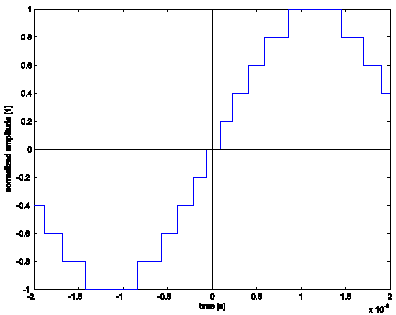
\includegraphics[width=4cm]{bilder/signal_quantisiert.png}
       	\end{center}
	\end{minipage}
\\
\hline

	\begin{minipage}[t]{9cm}
		\textbf{Analog} - \textit{zeit- und amplitudenkontinuierlich} \\

	\end{minipage}
	&
	\begin{minipage}[t]{9cm}
		\textbf{Digital} - \textit{zeitdiskret und quantisiert} \\

	\end{minipage}
\\
\hline
\end{tabular}
\renewcommand{\arraystretch}{\arraystretchOriginal}


	\subsection{Amplituden und Leistungen}
		\subsubsection{Normierte Signale}
			\begin{itemize}
				\item Absolute Werte des Signals sind irrelevant - Physikalische Dimension wird weggelassen.
				\item Signal $x(t)$ wird auf $|x_n(t)| \leq 1$ normiert.
			\end{itemize}
		\subsubsection{Signalbeschreibung}
			\begin{tabular}{p{4cm} p{4cm} p{4cm} p{4cm}}
				\textbf{Effektivwert} & 
				$x_{RMS} = \sqrt{P_x}$\\
				\textbf{Crestfaktor} & 
				$C = \dfrac{|x|_{pk}}{x_{RMS}}$\\
				\textbf{physikalische Leistung} &
				$P_{phys} = c \cdot P_x$\\
				& Bsp. $x(t) = i(t) \quad [A]$&
				$P_x = I_{RMS}^2 \quad [A^2]$&
				$P_{phys} = R \cdot I_{RMS}^2 \quad [W]$
			\end{tabular}
			 
			

	\subsection{Pegel (Dezibel)}
		\textbf{Mit Dezibel (dB) vergleicht man Leistungspegel, nicht Amplituden!}

	\subsubsection{Relative Pegel}
		\begin{tabbing}
			xxxxxxxxxxxxxxxxxxxxxxxxx \= xxxxxxxxxxxxxxxxxxxxxxx  \= xxxxxxxxxxxxxxxxxxxxxxx \=\kill
			\textbf{Spannungspegel} \> $L_U = 20 \cdot \log_{10} \frac{U_x}{U_0}$ \> $U_x = U_0 \cdot
			10^{\frac{L}{20}} $ \> $[L_U] = dB$ \\ 
			
			\textbf{Strompegel} \> $L_I  = 20 \cdot \log_{10} \frac{I_x}{I_0}$ \> $I_x = I_0 \cdot
			10^{\frac{L}{20}} $ \> $[L_I] = dB$ \\ 
			
			\textbf{Leistungspegel} \> $L_P = 10 \cdot \log_{10} \frac{P_x}{P_0}$ \> $P_x = P_0 \cdot
			10^{\frac{L}{10}} $ \> $[L_P] = dB$
		\end{tabbing}
		Beachte: Jeder relative Pegel gilt für U, I \& P. (Bei gleicher Referenz)
	

\subsubsection{Absolute Pegel}
	\begin{tabbing}
	xxxxxxxxxxxxxxxxxxxxxxxxx \= xxxxxxxxxxxxxxxxxxxxxxxxxxxxxxxxxxxxx  \= xxxxxxxxxxxxxxxxxxxxxxx \=\kill
	\textbf{dBW} \> Leistungspegel mit Bezugsgrösse $P_0 = $1W \> $\Longrightarrow \: 0 \: dBW = 1W = P_{0_{dBW}}$\\
	\textbf{dBm} \> Leistungspegel mit Bezugsgrösse $P_0 = $1mW \> $\Longrightarrow \: 0 \: dBm = 1mW = P_{0_{dBm}}$\\
	\textbf{dBV} \> Spannungspegel mit Bezugsgrösse $U_0 = $1V \> $\Longrightarrow \: 0 \: dBV = (1V)^2/R_{ref} = P_{0_{dBV}}$\\
	\textbf{dB}$\mu$V \> Spannungspegel mit Bezugsgrösse $U_0 = $1$\mu$V \> $\Longrightarrow \: 0 \: dB \mu V = (1 \mu V)^2/R_{ref} = P_{0_{dB\mu V}}$
	\end{tabbing}
Bei Leistungen in Bezug zu absoluten \textbf{Spannungspegeln} (dBV, dB$\mu$V) muss immer der \textbf{Referenz-Widerstand} ($R_{ref}$) berücksichtigt werden: \\
In der \textbf{HF-Technik} üblich, $R_{ref} = 50 \Omega \Rightarrow 0 dBV = 20 mW \qquad $
In der \textbf{Telefonie} üblich, $R_{ref} = 600  \Omega \Rightarrow 0 dBV =
1.67 mW$ 

\subsection{Fourier-Theorie}
	Die ganze Theorie zu den Fourier-Reihen, sowie zu der Fourier-Transformation sind in der Zusammenfassung des Moduls \textbf{Integral Transformation} zu finden.

\subsubsection{Ergänzung für NaT}
	\textbf{Symmetrie-Eigenschaft}\\
		Jedes Signal $x(t)$ kann aufgespaltet werden in:
		\parbox{6.5cm}{
			\begin{itemize}
				\item einen geraden (even) Anteil $x_e(t)$
				\item einen ungeraden (odd) Anteil $x_o(t)$
			\end{itemize}
		}
		$\qquad \Rightarrow x(t) = x_e(t) + x_o(t)$\\
		Es gilt:  $\quad$
		\parbox[t]{7cm}{
			$x_e(-t) = x_e(-t) : \qquad X_e(\omega)$ ist reellwertig\\
			\hspace{1cm} $x_o(-t) = -x_o(t) : \qquad X_o(\omega)$ ist imaginär
		}\\
		
	\begin{minipage}[t]{9cm}
		\textbf{Sinusf\"ormige Funktionen im Frequenzbereich}\\ 
			\hspace*{0.5cm}
			\parbox{8cm}{
				$\cos(\omega_0t) \laplace \pi \cdot (\delta(\omega - \omega_0)+ (\delta(\omega + \omega_0))$\\
				$\sin(\omega_0t) \laplace -j\pi \cdot (\delta(\omega - \omega_0)- (\delta(\omega + \omega_0))$	
			}
	\end{minipage}
	\begin{minipage}[t]{9cm}
		\textbf{Spektrum periodischer Leistungssignale}\\ 
			\hspace*{0.5cm}
			\parbox[b][1.2cm][c]{8cm}{
				$$\sum_{n = -\infty}^{+\infty} c_n \cdot e^{jn\omega_0t} \laplace 2\pi \sum_{n = -\infty}^{+\infty} c_n\delta(\omega - n\omega_0)$$		
			}
	\end{minipage}